% Shadow-feature selection under class imbalance.
% Build with ./build.sh (paper.pdf: preprint; build/paper_anonymous.pdf: TMLR submission).
\documentclass[10pt]{article}
\ifdefined\anonymous
  \usepackage{tmlr}
\else
  \usepackage[preprint]{tmlr}
\fi

\usepackage{amsmath,amssymb,amsthm,mathtools}
\usepackage{bm}
\usepackage{booktabs}
\usepackage{longtable}
\usepackage{multirow}
\usepackage{graphicx}
\usepackage{xcolor}
\usepackage{enumitem}
\usepackage{caption}
\usepackage{subcaption}
\usepackage[hidelinks]{hyperref}
\usepackage{url}
\usepackage[capitalise,noabbrev]{cleveref}
\usepackage{siunitx}
\sisetup{group-separator={,},group-minimum-digits=4}

\graphicspath{{../figures/}}

% ---------------------------------------------------------------- statements
\theoremstyle{plain}
\newtheorem{theorem}{Theorem}
\newtheorem{proposition}{Proposition}
\newtheorem{corollary}{Corollary}
\newtheorem{conjecture}{Conjecture}
\newtheorem{lemma}{Lemma}
\theoremstyle{definition}
\newtheorem{definition}{Definition}
\theoremstyle{remark}
\newtheorem{remark}{Remark}
\crefname{conjecture}{Conjecture}{Conjectures}
\crefname{proposition}{Proposition}{Propositions}

% ---------------------------------------------------------------- notation
\newcommand{\nmin}{n_{\min}}
\newcommand{\phat}{\hat p}
\newcommand{\sauc}{s_{\mathrm{AUC}}}
\newcommand{\E}{\mathbb{E}}
\renewcommand{\P}{\mathbb{P}}
\newcommand{\Gain}{\operatorname{Gain}}
\newcommand{\Bin}{\operatorname{Binomial}}
\newcommand{\logit}{\operatorname{logit}}
\newcommand{\AUC}{\operatorname{AUC}}
\newcommand{\FNR}{\mathrm{FNR}}
\newcommand{\FPR}{\mathrm{FPR}}
\newcommand{\code}[1]{\texttt{#1}}
\newcommand{\pkg}{\code{shadowselect}}

% Code location: withheld in the anonymous submission.
\ifdefined\anonymous
  \newcommand{\coderef}{the supplementary material}
  \newcommand{\repourl}{\textit{(repository URL withheld for double-blind review)}}
\else
  \newcommand{\coderef}{\url{https://github.com/Daniellopesba/shadow-feature-selection}}
  \newcommand{\repourl}{\url{https://github.com/Daniellopesba/shadow-feature-selection}}
\fi

% Numbers computed from results/ by experiments/paper_numbers.py
\InputIfFileExists{generated/numbers}{}{}

\setlist{itemsep=1pt,topsep=3pt,parsep=0pt,leftmargin=*}
\captionsetup{font=small,labelfont=bf}


\title{Shadow-Feature Selection Under Class Imbalance:\\ How the Minority Count Limits What Can Be Found}

\author{\name Daniel Lopes}

\def\month{MM}
\def\year{YYYY}
\def\openreview{\url{https://openreview.net/forum?id=XXXX}}

\begin{document}
\maketitle

\begin{abstract}
Shadow-feature selection keeps a feature when its importance beats that of artificial noise columns, usually row-permuted copies of the real features; Boruta is the best-known version. With a rare positive class this recipe drops features that do predict the target. We show that what controls the loss is the number of minority-class samples $\nmin$ combined with the effect size, and not the imbalance ratio. For the first tree of a gradient-boosted ensemble we prove that the split gain is Pearson's chi-square statistic, that as the prevalence goes to zero with $\nmin$ fixed the root split depends on the data only through $\nmin$ and the placement of the positives among the negatives, and that on a fixed range of thresholds its power depends only on $s = \nmin\delta^2$ for a standardised mean difference $\delta$. The false positive level of the max-shadow rule is $1/(K+1)$ for $K$ shadows at any imbalance, so imbalance takes away power and leaves the level unchanged. A rank test built from the same counting process has power that depends only on a rank analogue of $s$ for any continuous feature, and is more efficient than any single split for Gaussian-like features. We also show that the default intercept of XGBoost 1.x and 2.x adds a toll of order $\lambda/\hat p$ to every split. Simulations against acceptance criteria fixed in advance agree with every proved statement, and full ensembles fail at least as often as the root-split theory predicts. Across fourteen selection methods, eight departures from the Gaussian model and five real tables, a Mann--Whitney screen loses the fewest relevant features at the same false positive rate when the signal shifts the class distributions, and misses signals carried only by spread or by interactions, which trees find. We give guidance in terms of $\nmin$ and a scikit-learn compatible package.
\end{abstract}

\section{Introduction}\label{sec:intro}

A common feature-selection recipe in applied machine learning is to add columns that are known to be useless and keep the real features that beat them. The useless columns, called \emph{shadow features}, are random noise or copies of real features with their rows shuffled, which breaks any link to the target. After fitting a model, usually tree-based, any real feature whose importance falls below the largest shadow importance is dropped. Boruta \citep{kursa2010boruta} turns this into a procedure that repeats the comparison over many rounds and applies a binomial test to each feature's win count; BorutaPy \citep{homola2015borutapy} is its common Python implementation and BorutaSHAP \citep{keany2020borutashap} replaces impurity importance with SHAP values. Many teams also use the one-shot version directly on the gain importance of a gradient-boosted model. The appeal is that the shadows calibrate the threshold automatically: whatever importance pure noise can reach is, by construction, the bar to clear.

Credit default, fraud, medical diagnosis and churn all have rare positive classes, and in this setting the recipe drops features that do predict the target. This paper explains when and why, and what to do instead. The quantity that matters is the number of minority-class samples $\nmin$, combined with a feature's effect size. For a feature whose mean differs by $\delta$ within-class standard deviations between the classes, the combination is the \emph{scaling variable} $s = \nmin\delta^2$; for features of any distribution, a rank version $\sauc$ computed from the feature's ROC area plays the same role. A credit model with 5\% defaults among 1{,}000 loans and a fraud model with 0.1\% fraud among 50{,}000 transactions both have $\nmin = 50$, and to first order face the same difficulty.

The mechanism is not that noise features gain importance as the prevalence falls. The shadow rule keeps an irrelevant feature with probability at most $1/(K+1)$ for $K$ shadows at any imbalance (\cref{prop:level}). What changes is the advantage of an informative feature, which at the first split grows with $s$ while the best split pure noise can find depends on $\nmin$ alone and grows only slowly with it. Imbalance therefore takes away power and leaves the false positive level unchanged.

\paragraph{Contributions.}
\begin{enumerate}
\item \emph{Theory for the first split and for the shadow comparison (\cref{sec:theory}).} In the limit of small prevalence, the root split of a gradient-boosted tree depends on the data only through $\nmin$ and the positives' placement among the negatives (\cref{thm:limit}); for small effects on a fixed threshold window, only through $s$ (\cref{thm:scaling}). On XGBoost's full threshold range we conjecture, with numerical evidence, a slow $\log\log\nmin$ drift (\cref{conj:drift}). The shadow rule's level is $1/(K+1)$ for any learner whose importances depend on ranks, provided columns are continuous; per-feature shadows extend this to discrete columns (\cref{prop:level}). A rank test uses the same counting process as the split, has power that depends only on $\sauc$ for any continuous feature (\cref{prop:mw}), and is more efficient than any fixed split for Gaussian-like features but not for heavy-tailed or skewed ones (\cref{cor:efficiency}). XGBoost 1.x and 2.x intercepts add a toll of order $\lambda/\phat$ to every split (\cref{prop:toll}); 3.x does not.
\item \emph{Experiments that test each statement against pre-stated acceptance criteria (\cref{sec:experiments}, \cref{app:agreement}),} including the residual effect of the prevalence at fixed $\nmin$, which is real at weak signal.
\item \emph{A comparison of selection methods at both error rates (\cref{sec:methods}),} with SHAP and total-gain importances, BorutaPy, out-of-fold permutation importance, model-X knockoffs, $\ell_1$ and stability selection, and a rank-test screen, on synthetic data, on eight departures from the Gaussian model, and on five real tables with known null columns.
\item \emph{Guidance and a tested, scikit-learn compatible package (\cref{sec:guidance}),} \pkg{}, with an imbalance diagnostic, a rank-test screen and a Boruta-style selector. Every number and figure is produced by scripts in the repository with fixed seeds.
\end{enumerate}

\paragraph{What is classical and what is new.} Several ingredients are classical, and we credit them where they appear: the first-tree gain is Rao's score statistic, which for a binary split is Pearson's $X^2$ (\cref{prop:chi2}); the null best split is a maximally selected chi-square statistic, and its limit under local alternatives is the Brownian-bridge limit of \citet{miller1982maximally} and \citet{lausen1992maximally} (\cref{thm:scaling}); the level of the shadow rule is the Monte Carlo test argument of \citet{barnard1963discussion} and \citet{besag1989generalized} (\cref{prop:level}); and the efficiency of a fixed split relative to the rank test is the Pitman efficiency of the median test \citep{mood1954asymptotic}. New are the limit with the minority count fixed and the prevalence going to zero, which identifies $\nmin$ rather than $n$ as the sample size of the comparison; the scaling variables $s$ and $\sauc$ as the quantities that set the shadow rule's power; the intercept toll; per-feature shadows for discrete columns; and the assembly of these results into an account of shadow-based selection under imbalance, tested quantitatively.

\subsection{Related work}\label{sec:related}

\paragraph{Shadow, probe and knockoff methods.} Judging features against artificial ones that are irrelevant by construction predates Boruta: random probes \citep{stoppiglia2003ranking}, pseudo-variables that calibrate a selection threshold \citep{wu2007controlling}, artificial contrasts for tree ensembles \citep{tuv2009feature}, and pseudo-data that correct the bias of Gini importance \citep{sandri2008bias}. Boruta \citep{kursa2010boruta,kursa2011all} introduced permuted shadow copies with a random forest and a repeated binomial test, aimed at \emph{all-relevant} selection in the sense of \citet{nilsson2007consistent}; \citet{rudnicki2015all} review all-relevant methods. Benchmarks of Boruta against other random-forest selection methods, such as Vita \citep{janitza2018computationally}, VSURF \citep{genuer2010variable} and the method of \citet{hapfelmeier2013new}, include \citet{kursa2014robustness}, \citet{degenhardt2019evaluation} and \citet{speiser2019comparison}; none of them varies the minority count. Model-X knockoffs \citep{candes2018panning,barber2015controlling} compare each feature with its own synthetic copy and control the false discovery rate, so they do not pay the maximum-over-$K$ price of \cref{cor:shadows}; their power still depends on the importance statistic. Stability selection \citep{meinshausen2010stability,shah2013variable} controls false selections by subsampling a sparse model.

\paragraph{Feature importance in trees.} Impurity importances are biased toward features with many split points \citep{strobl2007bias} and can be analysed exactly for totally randomised trees \citep{louppe2013understanding}; debiased and out-of-sample versions exist \citep{li2019debiased,adler2022feature,zhang2023unbiased,scornet2023trees}. Permutation importance on out-of-bag or held-out data avoids the training-set bias \citep{breiman2001random,strobl2007bias}, can be made conditional \citep{strobl2008conditional}, and can be turned into p-values against a permutation null \citep{altmann2010permutation}. TreeSHAP gives consistent attributions, unlike the gain importance \citep{lundberg2017unified,lundberg2020local}. Split-selection bias motivates selecting splits by p-values rather than raw gain \citep{loh1997split,hothorn2006unbiased,strobl2007unbiased,nembrini2018revival}. Closest to our setting, \citet{janitza2013auc} show that error-rate permutation importance fails with a rare class and propose an AUC-based version, and balanced random forests keep every positive in every tree \citep{chen2004using}. These works address imbalance through the importance measure; we analyse how the minority count limits any shadow comparison.

\paragraph{Maximally selected statistics and rank tests.} The best split of a null feature is a maximally selected chi-square statistic \citep{miller1982maximally,lausen1992maximally,hothorn2003exact,hothorn2008generalized}. The placement values that represent the positives in our limit are standard in ROC analysis \citep{hanley1982meaning,delong1988comparing,pepe2004placement}. The loss from splitting a continuous variable at one threshold is the classical efficiency of grouping \citep{cox1957note} and of the median test relative to the Wilcoxon test \citep{mood1954asymptotic,mann1947test,hodges1956efficiency}.

\paragraph{Imbalanced learning.} Resampling, such as SMOTE \citep{chawla2002smote}, cost-sensitive learning and ensembles are surveyed by \citet{fernandez2018learning}. That literature targets predictive performance rather than the reliability of feature selection.

\section{Setup}\label{sec:setup}

\paragraph{Data.} We observe $n$ samples $(x_i, y_i)$ with $x_i\in\mathbb R^d$ and $y_i\in\{0,1\}$, labelling the minority class 1. The \emph{minority count} is $\nmin = \sum_i y_i$ and the prevalence is $\phat = \nmin/n$. A feature $X_j$ is \emph{relevant} if it is not independent of $Y$ and \emph{irrelevant} otherwise; the level results of \cref{sec:level} need the stronger condition that $X_j$ is independent of $Y$ and of all other candidates (a \emph{strong null}). Unless stated otherwise the experiments use a Gaussian location-shift model with exactly $\nmin = \operatorname{round}(np)$ positives: $d_{\text{rel}}$ relevant features with $X_j\mid Y{=}0\sim N(0,1)$ and $X_j\mid Y{=}1\sim N(\delta,1)$, and $d_{\text{null}}$ strong-null features $X_j\sim N(0,1)$, all mutually independent given $Y$. \Cref{sec:robustness} departs from this model in eight ways and \cref{sec:realdata} uses real tables.

\paragraph{Effect size.} $\delta$ is the mean difference in units of the within-class standard deviation; $\delta = 0.3$, 0.5 and 1 give single-feature ROC areas of 0.58, 0.64 and 0.76. The \emph{scaling variable} of a feature is $s = \nmin\delta^2$, the minority count times the squared effect size. Because a standardised mean difference has no fixed meaning for skewed or discrete features, we also use the \emph{rank scaling variable} $\sauc = 4\pi\,\nmin(\AUC - \tfrac12)^2$, where $\AUC$ is the feature's single-feature ROC area; in the Gaussian model $\sauc \approx s$ (\cref{sec:rank}).

\paragraph{The shadow rule.} Let $C$ be the candidate features and $S$ a set of $K$ \emph{shadows}: artificial columns generated independently of $Y$, here row-permutations of candidate columns. Fit a model on $C\cup S$ and compute an importance $I_j$ for every column. The \emph{one-shot max-shadow rule} keeps candidate $j$ if $I_j > \max_{k\le K} I_{s_k}$; a quantile $q < 1$ of the shadow importances gives a laxer rule. \emph{Boruta-style selection} \citep{kursa2010boruta} repeats the comparison over $R$ rounds with fresh shadows, counts each candidate's wins (hits), and tests the count against $\Bin(R,\tfrac12)$ in both directions with a Bonferroni correction over candidates: a significantly high count accepts the feature, a significantly low count rejects it, and anything in between is \emph{tentative}. Boruta itself uses $K = d$ shadows (one per candidate) and removes rejected features as it goes; BorutaPy \citep{homola2015borutapy} does the same with a two-step multiple-testing correction.

\paragraph{Error rates.} The \emph{false negative rate} (FNR) is the fraction of relevant candidates dropped; the \emph{false positive rate} (FPR) is the fraction of irrelevant candidates kept. In the main sweep (\cref{sec:exp-ensemble}) the strong-null columns in the data serve as the shadows, so only FNR is defined; the method comparison (\cref{sec:methods}) separates irrelevant candidates from method-built shadows and reports both.

\paragraph{Importances.} For gradient-boosted trees we use training-set importances. XGBoost's default \code{importance\_type="gain"} is the \emph{mean} split gain \eqref{eq:gain} over the splits that use a feature, \code{total\_gain} the sum; \code{feature\_importances\_} normalises the chosen type to sum to one. Random forests and scikit-learn's gradient boosting report the normalised impurity decrease. We also use mean absolute TreeSHAP values \citep{lundberg2020local}, the statistic of BorutaSHAP \citep{keany2020borutashap}, and permutation importance on held-out data.

\paragraph{Learner.} Unless stated otherwise the learner is \code{xgboost.XGBClassifier} 2.1.3 with 300 trees of depth 6, learning rate 0.1, \code{tree\_method="hist"}, $\lambda = 1$, $\gamma = 0$, \code{min\_child\_weight}${}=1$ and no early stopping: reasonable defaults of the kind used inside selection loops. The intercept is the \emph{prevalence intercept} $b = \phat$, which is XGBoost's default from version~3.0; \cref{sec:gain} explains why the default of earlier versions matters, and \cref{app:intercept-arm} reports the experiments with the 2.x default.

\section{Theory}\label{sec:theory}

Propositions, theorems and corollaries are proved (long proofs in \cref{app:proofs}). A \emph{numerical evaluation} computes, by Monte Carlo on the limit object and not on XGBoost, a quantity that a proved limit defines exactly. A \emph{conjecture} is not proved, and a \emph{heuristic} motivates an experiment but is not used as evidence. The proved results cover the \emph{first tree} of a gradient-boosted ensemble with log-loss (\cref{sec:gain,sec:limit,sec:scaling}), the shadow comparison for any learner whose importances depend on ranks (\cref{sec:level}), and a rank test on the same data (\cref{sec:rank}); for the full ensemble we state a conjecture (\cref{sec:ensemble}).

\paragraph{Scope.} We analyse XGBoost's second-order split criterion with \emph{exact greedy} search over all midpoints. XGBoost's default \code{hist} search uses at most 255 quantile cuts; \cref{app:hist} extends the limit theorem to it under an assumption on the quantile sketch. LightGBM \citep{ke2017lightgbm} uses the same criterion with a prevalence intercept.

\subsection{The split gain in the first tree}\label{sec:gain}

For log-loss with raw score $F$ and $\sigma(F) = 1/(1+e^{-F})$, the gradient and Hessian of sample $i$ are $g_i = \sigma(F_i) - y_i$ and $h_i = \sigma(F_i)(1-\sigma(F_i))$. Before the first tree every sample has the score $F^{(0)} = \logit(b)$, where the \emph{base score} $b$ is the initial predicted probability, so $h_i = b(1-b)$ is constant in the whole first tree. For a set of samples $S$ write $G_S = \sum_{i\in S} g_i$, $H_S = \sum_{i\in S} h_i$, $n_S = |S|$ and $k_S$ for its number of positives. Splitting node $S$ into $L$ and $R$ has gain
\begin{equation}\label{eq:gain}
  \Gain = \frac{G_L^2}{H_L+\lambda} + \frac{G_R^2}{H_R+\lambda} - \frac{G_S^2}{H_S+\lambda},
\end{equation}
and the split is made only if $\Gain > \gamma$ and $H_L, H_R \ge w$, where $\lambda$ (default 1), $\gamma$ (default 0) and $w$ (\code{min\_child\_weight}, default 1) are XGBoost's regularisation parameters. \Cref{eq:gain} is what the software computes, compares with $\gamma$ and reports (\citet{chen2016xgboost} write half of it).

\begin{proposition}[the first-tree gain is Pearson's chi-square]\label{prop:chi2}
In the first tree, with $\lambda = 0$, the gain of splitting a node $S$ with $0 < k_S < n_S$ into non-empty children is
\begin{equation}\label{eq:chi2}
  \Gain = \frac{\phat_S(1-\phat_S)}{b(1-b)}\,X_S^2,\qquad X_S^2 = \frac{n_S\,(k_L n_R - k_R n_L)^2}{n_L\,n_R\,k_S\,(n_S-k_S)},
\end{equation}
where $\phat_S = k_S/n_S$ and $X_S^2$ is Pearson's chi-square statistic (without continuity correction) for the $2\times 2$ table of child by class. At the root with $b = \phat$ the factor is 1 and $\Gain = X^2$.
\end{proposition}

\begin{proof}
With constant Hessian $h$, $H_T = h\,n_T$. For reals $a, c$ and $x, y > 0$, $a^2/x + c^2/y - (a+c)^2/(x+y) = (ay-cx)^2/(xy(x+y))$. Taking $a = G_L$, $c = G_R$, $x = hn_L$, $y = hn_R$ gives $\Gain = (G_L n_R - G_R n_L)^2/(h\,n_L n_R n_S)$. Since $G_T = b\,n_T - k_T$, the terms in $b$ cancel and $G_L n_R - G_R n_L = k_R n_L - k_L n_R$. Multiply and divide by $\phat_S(1-\phat_S) = k_S(n_S-k_S)/n_S^2$.
\end{proof}

This is the classical fact that, with a constant Hessian, the Newton gain at the null fit is Rao's score statistic for the split indicator, which for a binary indicator is Pearson's $X^2$ \citep{rao1948large,agresti2013categorical,zeileis2008model}. It turns the gain into a test statistic whose null law can be studied as $\nmin$ varies.

\paragraph{The intercept, by XGBoost version.} We measured the default base score (\cref{tab:intercepts}): $b = 1/2$ in XGBoost~1.x; one Newton step from $F = 0$ in 2.0--2.1, so $b = \sigma(4\phat-2) \to 0.119$ as $\phat \to 0$; and the prevalence $b = \phat$, which makes the root gradient sum zero, from 3.0. We call $b = \phat$ the \emph{prevalence intercept}. When $b \ne \phat$, every split pays a toll.

\begin{table}[t]
\centering\small
\caption{XGBoost's default base score $b$ after fitting, by version and prevalence (identical for \code{exact} and \code{hist}), and the chi-square a first-tree split needs before its gain is positive (\cref{prop:toll}, approximation \eqref{eq:approx}, valid when both children have $H_c\gg\lambda$ and are not enriched in positives; $\lambda = 1$).}\label{tab:intercepts}
\begin{tabular}{lcccccc}
\toprule
 & \multicolumn{3}{c}{default $b$} & \multicolumn{3}{c}{$X^2$ needed for $\Gain > 0$} \\
\cmidrule(lr){2-4}\cmidrule(lr){5-7}
XGBoost & $\phat = 0.001$ & $0.01$ & $0.1$ & $\phat = 0.001$ & $0.01$ & $0.1$\\
\midrule
1.7.6 & 0.5 & 0.5 & 0.5 & 997.0 & 97.0 & 7.11 \\
2.1.3 & 0.1196 & 0.1235 & 0.1680 & 133.8 & 12.0 & 0.37 \\
3.1.3 & 0.001 & 0.01 & 0.1 & 0 & 0 & 0 \\
\bottomrule
\end{tabular}
\end{table}

\begin{proposition}[the intercept toll]\label{prop:toll}
Let $b \ne \phat$ in the first tree and $r = (b-\phat)/(b(1-b))$, the root's gradient-to-Hessian ratio. If both children have $H_c \gg \lambda$ and are not enriched in positives ($|\phat_c - \phat| \ll |b - \phat|$), then
\begin{equation}\label{eq:approx}
  \Gain \approx \frac{\phat(1-\phat)}{b(1-b)}\,X^2 - \lambda r^2,
\end{equation}
with the exact identity \eqref{eq:toll} and the remainder bound \eqref{eq:remainder} of \cref{app:proof-toll}. Such a split has positive gain only if
\begin{equation}\label{eq:threshold}
  X^2 > \lambda\,\frac{(b-\phat)^2}{b(1-b)\,\phat(1-\phat)}
  \;\approx\; \begin{cases} e^{-2}\lambda/\phat & \text{XGBoost 2.0--2.1},\\ \lambda/\phat & \text{XGBoost 1.x},\end{cases}\qquad \phat \to 0.
\end{equation}
\end{proposition}

With the 2.x default at $\phat = 0.001$ such a split needs $X^2 > 134$, so the first tree is often a single leaf, and the splits that pass are small children enriched in positives, which any continuous column can produce (\cref{prop:mcw}; experiments in \cref{app:intercept-arm}).

\subsection{The small-prevalence limit}\label{sec:limit}

Fix a feature and let $F_0$ and $F_1$ be its distribution functions among negatives and positives. The \emph{placement value} of a positive with feature value $x$ is $V = F_0(x)$, the fraction of negatives below it; its distribution function $G(u) = \P(V \le u)$ describes how the positives sit among the negatives \citep{hanley1982meaning,pepe2004placement}. A feature is irrelevant if $G(u) = u$. In the Gaussian model $V = \Phi(Z)$ with $Z \sim N(\delta,1)$, so $G(u) = \Phi(\Phi^{-1}(u) - \delta)$.

The root split takes the best threshold of every feature and then the best feature. Index thresholds by the fraction $u = n_L/n$ of samples sent left. With the prevalence intercept the left child's gradient sum is $\nmin u - k_L$, $H_L = \nmin u(1-\phat)$ and $H_R = \nmin(1-u)(1-\phat)$, so the gain as a function of $u$ is
\begin{equation}\label{eq:process}
  \Gain(u) = \bigl(k_L(u) - \nmin u\bigr)^2\left[\frac{1}{\nmin u(1-\phat)+\lambda} + \frac{1}{\nmin(1-u)(1-\phat)+\lambda}\right],\qquad u \in [u_w, 1-u_w],
\end{equation}
with $u_w = w/(\nmin(1-\phat))$. Apart from the counting process $k_L(u)$, everything is a function of $\nmin$, $\phat$, $\lambda$ and $w$.

\begin{theorem}[small-prevalence limit]\label{thm:limit}
Condition on the labels: given them, each feature's $\nmin$ positive values are i.i.d.\ $F_1$ and its $n-\nmin$ negative values i.i.d.\ $F_0$, independently, and features are independent of one another. Let each $F_0$ be continuous and each placement value $V = F_0(X)$, $X\sim F_1$, atomless (equivalently, $F_1$ has no atoms and gives no mass to any interval on which $F_0$ is constant, including the interval below the support of $F_0$). Use the prevalence intercept, exact greedy search, and $w > 0$ with $\nmin > 2w$. Fix $\nmin$, $\lambda$, $w$ and the features' laws, and let $n \to \infty$, so $\phat \to 0$. Then the gain processes \eqref{eq:process} of the features converge in distribution, jointly and independently across features, to
\begin{equation}\label{eq:limit}
  \Gamma(u) = \bigl(N(u) - \nmin u\bigr)^2\left[\frac{1}{\nmin u+\lambda} + \frac{1}{\nmin(1-u)+\lambda}\right],\qquad u\in[w/\nmin,\,1-w/\nmin],
\end{equation}
where $N(u) = \#\{i \le \nmin : V_i \le u\}$ for i.i.d.\ placements $V_1,\dots,V_{\nmin}$ with law $G$. The same holds for shadows, which are row-permutations of candidate columns and so are not conditionally independent of their sources: a shadow's limit process is that of a null feature, independent of all the others (\cref{lem:shadow} in \cref{app:proof-limit}). The convergence is in the Skorokhod $J_1$ topology for the counting processes and uniform for the gains after a time change that tends to the identity. The suprema $M_j = \sup_u \Gamma_j(u)$ converge jointly, and their law depends only on $\nmin$, $\lambda$, $w$ and the placement laws $G_j$.
\end{theorem}

The proof (\cref{app:proof-limit}) uses that a positive's rank fraction among all $n$ values converges to $V_i$, because the negatives' empirical distribution function converges uniformly to $F_0$. For a null feature \eqref{eq:limit} is the maximally selected chi-square statistic of $\nmin$ uniform points \citep{miller1982maximally,lausen1992maximally}; what is specific here is that its sample size is $\nmin$, not $n$. The law of $M$ has atoms, so features can tie, and XGBoost breaks ties by column order. Without regularisation ($\lambda = w = 0$) the null supremum has infinite mean and diverges as $\nmin \to \infty$ \citep{jaeschke1979asymptotic,donoho2004higher}; $w$ and $\lambda$ keep it small.

\subsection{The scaling variable \texorpdfstring{$s = \nmin\delta^2$}{s}}\label{sec:scaling}

At a fixed threshold $u$, $N(u)$ is binomial and the standardised deviation $(N(u)-\nmin u)^2/(\nmin u(1-u))$ has non-centrality $\nu(u) = \nmin(G(u)-u)^2/(u(1-u))$; in the Gaussian model $\max_u\nu(u)/(\nmin\delta^2) \to 2/\pi$ as $\delta\to 0$, at the median split (\cref{prop:fixed} in \cref{app:fixed}). So the signal at a fixed threshold is governed by $s = \nmin\delta^2$. The best threshold is chosen from the data, and the null competitors are maxima too; the next theorem accounts for both.

\begin{theorem}[the scaling variable, on a fixed window]\label{thm:scaling}
In the Gaussian model, let $\nmin \to \infty$ and $\delta \to 0$ with $\nmin\delta^2 \to s \in [0,\infty)$ (take $\delta \ge 0$), after the limit $n\to\infty$ of \cref{thm:limit}. Fix $\lambda \ge 0$, $w > 0$ and a window $[\varepsilon, 1-\varepsilon]$ with $0 < \varepsilon < 1/2$. On that window, the limit gain processes \eqref{eq:limit} of independent features converge jointly and uniformly in distribution to independent copies of
\begin{equation}\label{eq:bridge}
  \Gamma^{(s)}(u) = \frac{\bigl(\mathbb B(u) - \sqrt s\,\psi(u)\bigr)^2}{u(1-u)},\qquad \psi(u) = \varphi\bigl(\Phi^{-1}(u)\bigr),
\end{equation}
where $\mathbb B$ is a Brownian bridge and $s$ is the feature's own scaling variable ($s = 0$ for a null feature). Consequently, if thresholds are restricted to the window, the probability that an informative feature's best split beats the best splits of $K$ null features converges to
\[
  \omega_\varepsilon(s,K) = \P\Bigl(\sup_{[\varepsilon,1-\varepsilon]}\Gamma^{(s)} > \max_{k\le K}\,\sup_{[\varepsilon,1-\varepsilon]}\Gamma^{(0)}_k\Bigr),
\]
which depends on $s$, $K$ and $\varepsilon$, and not on $\lambda$, $w$ or how $\nmin$ and $\delta$ combine to give $s$. It is non-decreasing in $s$, and $\omega_\varepsilon(0,K) = 1/(K+1)$.
\end{theorem}

The proof (\cref{app:proof-scaling}) splits $N(u) - \nmin u$ into a uniform empirical process and a drift $-\sqrt s\,\psi(u)$; monotonicity is Anderson's inequality \citep{anderson1955integral}. The limit is classical under contiguous alternatives \citep{miller1982maximally,lausen1992maximally,hothorn2008generalized}; what it adds is that $s = \nmin\delta^2$ sets the shadow rule's power at the root, so halving $\delta$ costs as much as dividing $\nmin$ by four. For a location family with standardised density $f$ and distribution function $F$, $\psi$ becomes the density-quantile function $J_f(u) = f(F^{-1}(u))$. XGBoost, however, searches the window $[w/\nmin, 1-w/\nmin]$, which widens with $\nmin$; near its edges the drift vanishes while the null supremum keeps growing.

Numerically ($\lambda = w = 1$, $K = 9$), the root win probability at $s = 12.5$ is 0.85, 0.82, 0.79, 0.80 and 0.76 at $\nmin = 50$, 200, 1000, 5000 and 20{,}000, and flat at $0.86 \pm 0.01$ on the window $[0.1,0.9]$. So in practice $s$ fixes the root win probability to within about 0.1; \cref{app:conj1} conjectures that it is not sufficient asymptotically, with a $\log\log\nmin$ drift (\cref{conj:drift}).

\subsection{The shadow comparison: level, number of shadows and rounds}\label{sec:level}

The level of the shadow comparison holds for any sample size and number of trees under four conditions:
\begin{enumerate}[label=(A\arabic*),start=0]
  \item \emph{Exchangeable rows.} The rows are i.i.d.\ (or the rows of the column under test are exchangeable given $Y$ and the other columns).
  \item \emph{Rank dependence.} The importances are a function of $Y$, the columns' rank vectors and independent randomness. Trees with exact search satisfy this; for \code{hist} we checked it numerically only. Rank-transforming the columns makes it hold for any learner.
  \item \emph{Column symmetry.} Permuting the columns permutes the importances in law (shuffling the column order before each fit ensures this).
  \item \emph{Continuity.} No column has ties.
\end{enumerate}

\begin{proposition}[level of the shadow rule]\label{prop:level}
Assume (A0)--(A3). Let candidate $j$ be null in the strong sense that $X_j$ is independent of $(Y, X_{C\setminus j})$, and let each of the $K$ shadows be an independent, uniformly random row-permutation of some candidate column, or a column of i.i.d.\ continuous noise. Then
\[
  \P\Bigl(I_j > \max_{k\le K} I_{s_k}\Bigr) \le \frac{1}{K+1},
\]
with equality when importances tie with probability zero, for every $n$, $\nmin$, $\phat$ and number of trees. If all $K$ shadows are permutations of $X_j$ itself (\emph{per-feature shadows}), the same bound holds under (A0) and (A2) alone, for columns of any type.
\end{proposition}

The proof (\cref{app:proof-level}) is the Monte Carlo test argument \citep{barnard1963discussion,hope1968simplified,besag1989generalized}, as applied to random probes by \citet{stoppiglia2003ranking} and \citet{wu2007controlling}. Imbalance changes only the rule's \emph{power}. A null candidate correlated with a relevant one is not covered. With Boruta's shadows, discrete columns break exchangeability, as with the cardinality bias of impurity importance \citep{strobl2007bias}; per-feature shadows restore the level (\cref{sec:exp-level}).

\begin{corollary}[number of shadows, at the root]\label{cor:shadows}
In the limit of \cref{thm:limit}, let $M_j$ be an informative candidate's best root gain, $M_0$ a null feature's, and $Q(x) = \P(M_0 < x)$. Counting exact ties as losses, the probability that the root uses candidate $j$ rather than any of $K$ shadows is $\E[Q(M_j)^K]$, which is strictly decreasing in $K$ whenever $\P(0 < Q(M_j) < 1) > 0$.
\end{corollary}

\begin{proof}
By \cref{lem:shadow}, the $K$ shadow suprema converge to i.i.d.\ copies of $M_0$, independent of $M_j$. Given $M_j$ the candidate wins if every shadow is below it, which has probability $Q(M_j)^K$; take expectations.
\end{proof}

Boruta uses one shadow per candidate, so $K$ grows with the width of the table. At $\nmin = 50$, $\delta = 0.5$ the root win probability falls from 0.90 with $K = 5$ to 0.47 with $K = 200$.

\begin{proposition}[repeated rounds]\label{prop:rounds}
Run $R$ rounds on fixed data $D$, each with fresh shadows, a fresh column order and fresh learner randomness, without removing features between rounds, and let $\theta_j(D)$ be a null candidate's per-round hit probability given $D$. Its hit count is $T_j \mid D \sim \Bin(R, \theta_j(D))$ with $\E\,\theta_j(D) \le 1/(K+1)$ under the conditions of \cref{prop:level}. Let the candidate be rejected when $T_j \le r_R$, the largest $r$ with $\P(\Bin(R,\tfrac12) \le r) < \alpha/d$ (one-sided, Bonferroni over $d$ candidates), and $r_R = -1$ if there is none, in which case no candidate is rejected. Then the probability that it is kept is
\begin{equation}\label{eq:rounds}
  \P(\text{keep}) = \E\bigl[\P(\Bin(R,\theta_j(D)) > r_R)\bigr] \le \frac{R}{(K+1)(r_R+1)}\quad (r_R \ge 0),
\end{equation}
and, as $R\to\infty$ with $\alpha$, $d$ and $K$ fixed, $\limsup_R \P(\text{keep}) \le \P(\theta_j(D) \ge \tfrac12) \le \min\bigl\{2/(K+1),\ 4\operatorname{Var}\theta_j(D) + 4/(K+1)^2\bigr\}$.
\end{proposition}

The proof is in \cref{app:proof-rounds}. The keep rate depends on $R$, $K$ and $d$, not monotonically in $R$: with $K = 10$, $R = 20$ and a hit rate of $1/11$ it is 0.10 at $d = 10$ and 0.27 at $d = 200$ (\cref{tab:rounds-grid}). A Benjamini--Hochberg correction rejects every candidate Bonferroni rejects, so the bounds hold for it too.

\subsection{A rank test on the same data}\label{sec:rank}

The gain process \eqref{eq:limit} is built from the counting process $N$. So is the Mann--Whitney statistic. A feature's single-feature ROC area is $\AUC = \E V = \int_0^1 (1 - G(u))\,du$, the probability that a positive exceeds a negative. Define the \emph{rank scaling variable}
\begin{equation}\label{eq:sauc}
  \sauc = 4\pi\,\nmin\,(\AUC - \tfrac12)^2 .
\end{equation}
In the Gaussian model $\AUC = \Phi(\delta/\sqrt2)$, so $\sauc = s\,(1 + O(\delta^2))$; at $\delta = 0.5$, $\sauc = 0.96\,s$.

\begin{proposition}[the Mann--Whitney test in the same limit]\label{prop:mw}
In the setting of \cref{thm:limit}, the normalised Mann--Whitney statistic $W_n = U/(\nmin(n-\nmin))$ of a feature converges almost surely, on the coupling of \cref{app:proof-limit}, to
\begin{equation}\label{eq:mw}
  W = \frac{1}{\nmin}\sum_{i=1}^{\nmin} V_i = 1 - \frac{1}{\nmin}\int_0^1 N(u)\,du .
\end{equation}
If moreover $\nmin\to\infty$ along placement laws $G_{\nmin} \to \mathrm{id}$ uniformly with $\sauc \to s_*$ (the condition on $G_{\nmin}$ is needed: $V \equiv \tfrac12$ has $\sauc = 0$ but a degenerate $W$), then $\sqrt{12\nmin}\,(W - \tfrac12) \Rightarrow \mathcal N(\pm\sqrt{3 s_*/\pi},\,1)$, with the sign of $\AUC - \tfrac12$, and the two-sided test at level $\alpha$, with $z_{\alpha/2}$ the upper $\alpha/2$ quantile of the standard normal, has asymptotic power
\begin{equation}\label{eq:mwpower}
  \Phi\bigl(\sqrt{3s_*/\pi} - z_{\alpha/2}\bigr) + \Phi\bigl(-\sqrt{3s_*/\pi} - z_{\alpha/2}\bigr),
\end{equation}
for every pair of continuous class-conditional distributions.
\end{proposition}

So the rank test's power depends only on $\sauc$, whatever the feature's distribution (proof in \cref{app:proof-mw}); at finite $n$, $s_*$ becomes about $s_*(1-\phat)$. By \eqref{eq:mw}, the split takes the \emph{largest} standardised deviation of $N(u)$ from $\nmin u$, the rank test the \emph{average} one, with a known null law.

\begin{corollary}[efficiency of one split relative to the rank test]\label{cor:efficiency}
Let a feature follow a location family with bounded standardised density $f$, shift $\delta \to 0$ and $\nmin\delta^2 \to s$. A pre-specified threshold $u$, with $F^{-1}(u)$ uniquely defined and $f$ continuous there, has non-centrality $s\,J_f(u)^2/(u(1-u))$ (\cref{prop:fixed}), and the rank test has non-centrality $12 s\,(\int f^2)^2$ (\cref{prop:mw}, since $\AUC - \tfrac12 = \delta\int f^2 + o(\delta)$). The best fixed threshold, chosen knowing $f$, therefore has asymptotic relative efficiency
\begin{equation}\label{eq:efficiency}
  \mathrm{ARE}(f) = \frac{\sup_u J_f(u)^2/(u(1-u))}{12\,\bigl(\int f^2\bigr)^2}
\end{equation}
with respect to the rank test: $2/3$ for the normal, $3/4$ for the logistic, $0.85$ for $t_3$ and $4/3$ for the Laplace distribution (all at the median), and $4.8$ for the log-normal with $\sigma = 1$, at an interior maximiser $u \approx 0.01$ (the median split has $0.40$).
\end{corollary}

For the normal, $2/3$ is the Pitman efficiency of the median test \citep{mood1954asymptotic,hodges1956efficiency}: one fixed split needs 1.5 times as many positives as the rank test. For skewed features a well-placed split can win, though the log-normal value needs $\nmin u^* \gg 1$. The shadow rule also pays for searching thresholds; a numerical evaluation of the limits ($K = 9$, level $0.1$, $\nmin = 50$) gives:

\begin{center}\small
\begin{tabular}{lccccc}
\toprule
$s = \nmin\delta^2$ & 2 & 5 & 10 & 15 & 25\\
\midrule
max-shadow rule, best root split (limit \eqref{eq:limit}) & 0.27 & 0.51 & 0.77 & 0.90 & 0.98\\
fixed median split (non-centrality $2s/\pi$) & 0.31 & 0.56 & 0.81 & 0.93 & 0.99\\
Mann--Whitney (\cref{eq:mwpower}) & 0.40 & 0.71 & 0.93 & 0.98 & 1.00\\
\bottomrule
\end{tabular}
\end{center}

Power 0.9 needs $s \approx 9.0$ for the rank test, 13.5 for the median split and 15 for the max-shadow rule, in the same order at $\nmin = 25$ and 250. A rank test cannot see a feature that acts only through an interaction or its spread (\cref{sec:robustness}).

\subsection{The full ensemble}\label{sec:ensemble}

After the first tree the scores differ between samples and \cref{prop:chi2} no longer holds; we prove only an accounting identity (\cref{prop:accounting} in \cref{app:accounting}).

\begin{conjecture}[the full ensemble]\label{conj:ensemble}
Consider a boosted ensemble with the prevalence intercept, mean-gain importance (exact or \code{hist} search), and the one-shot max-shadow rule with ties counted as losses, in the Gaussian model. (a) For every $n$ with $\phat \le 0.1$, the false negative rate of an informative candidate is at least the root-split failure probability $1 - \E[Q(M_j)^K]$ of \cref{cor:shadows}, evaluated at the same $(\nmin, \delta, K, \lambda, w)$. (b) At fixed $\nmin$, $\delta$ and $K$, the false negative rate does not decrease as $\phat$ decreases (that is, as $n = \nmin/\phat$ grows).
\end{conjecture}

\Cref{sec:experiments} tests both parts cell by cell.

\section{Experiments: testing the theory}\label{sec:experiments}

Each statement of \cref{sec:theory} that a simulation can test was paired, before any comparison was computed, with a statistic, a prediction and a rule that turns the two into a verdict (\cref{app:agreement}). This section reports the comparisons that carry the argument; \cref{tab:agreement} lists all of them, and \cref{app:experiments} gives the remaining experiments.

\paragraph{Protocol.} All experiments use the model of \cref{sec:setup}. Every repeat draws a new data set from a seed derived from a hash of the scenario's parameters and the repeat index, so every number is reproducible bit for bit with the pinned library versions (\cref{app:reproducibility}). Where two arms of an experiment differ only in the learner's settings, such as the intercept, both arms use the same data sets. Standard errors are clustered by data set and error bars show two standard errors. \Cref{tab:experiments} summarises the designs.

\begin{table}[t]
\centering\small
\caption{Experiments. $K$ is the number of shadows; ``null features as shadows'' means that the strong-null columns of the data serve as the shadows, so only the false negative rate is defined.}\label{tab:experiments}
\begin{tabular}{@{}lp{0.70\textwidth}r@{}}
\toprule
 & Design & Data sets\\
\midrule
E1 & One depth-1 tree; 1 informative and 9 null features; $\nmin$ 10--1000, $p\in\{0.001, 0.01, 0.1\}$, $\delta$ 0.1--1; both intercepts; exact and \code{hist}; 100 repeats & 34{,}000\\
E2 & 300 trees; 5 relevant and 5 null features (null features as shadows, $K = 5$); $\nmin$ 10--2000, $p$ 0.001--0.2, $\delta\in\{0, 0.3, 0.5, 1\}$; both intercepts on the same data; also XGBoost 3.1 & \numEtwoFits\\
E3 & As E2, importances after $k = 1,\dots,300$ rounds & \numEthreeFits\\
E4 & 5 relevant and 5 irrelevant candidates, $K = 10$ method-built shadows, $\delta = 0.5$, $\nmin$ 10--500, $p\in\{0.01, 0.1\}$; 14 selection methods on the same data sets; 20 repeats & \numEfourFits\\
E5 & As E2 at $\delta = 0.5$ with LightGBM, random forests and scikit-learn gradient boosting & \numEfiveFits\\
E7 & E4 design, 60 Boruta rounds stored round by round & 6{,}000\\
E8 & One-shot rule with $K = 5$, 50 or 200 null features & 180\\
E9 & Eight departures from the Gaussian model (\cref{sec:robustness}) & \numEnineFits\\
E10 & Level with discrete columns: Boruta's and per-feature shadows & \numEtenFits\\
E11 & Five real tables with appended null columns (\cref{sec:realdata}) & \numEelevenFits\\
\bottomrule
\end{tabular}
\end{table}

\subsection{The first split}\label{sec:exp-first}

\paragraph{The gain is Pearson's chi-square, and the null law depends on $\nmin$ (P1--P3).} With $\lambda = 0$, exact search and the prevalence intercept, the root gain reported by XGBoost matches $X^2$ to a relative error of \numPoneErr, which is float32 precision. Under XGBoost's default regularisation, the median of a null feature's best split varies by at most \numPthreeSpread\% across $n = 10^3$ to $10^5$ at every $\nmin$ (\cref{fig:first}a), while it grows only slowly with $\nmin$. Without regularisation it grows with $n$, as remark (iii) after \cref{thm:limit} requires.

\paragraph{The limit predicts XGBoost's root decision (P4, P5).} \Cref{fig:first}b shows how often a depth-1 tree chooses the one informative feature over nine null ones, with the column order shuffled before every fit so that ties are broken at random. The curves are the limit \eqref{eq:limit}, computed by Monte Carlo without fitting anything. Over the \numPfourCells{} informative cells with the prevalence intercept and exact search, the mean absolute difference between prediction and measurement is \numPfourMAE{} and the goodness-of-fit test gives $p = \numPfourP$, so the data are consistent with the limit being exact at $\phat$ as large as 0.1 and $n$ as small as 250. Histogram search agrees as closely under assumption (H1) of \cref{cor:hist} (mean difference \numPfourMAEhist). At fixed $s$, the prevalence has no detectable effect on the root decision: a logistic regression of the per-run outcome on a spline of $\log s$ and on $\log_{10}\phat$ estimates a change of \numPfiveAME{} in the win probability per decade of $\phat$ (95\% interval \numPfiveLo{} to \numPfiveHi).

\paragraph{The intercept toll (P6).} Under the XGBoost~2.x default intercept at $\phat = 0.001$, $\nmin = 50$ and $\delta = 0.5$, exact search made no split at all in \numPsixNoSplitZeroZeroOne{} of runs; evaluating \eqref{eq:toll} on each run's own data predicts whether the first tree splits in \numPsixAgree\% of the 300 runs of this cell. \Cref{fig:toll} in \cref{app:intercept-arm} shows the toll across cells.

\begin{figure}[t]
\centering
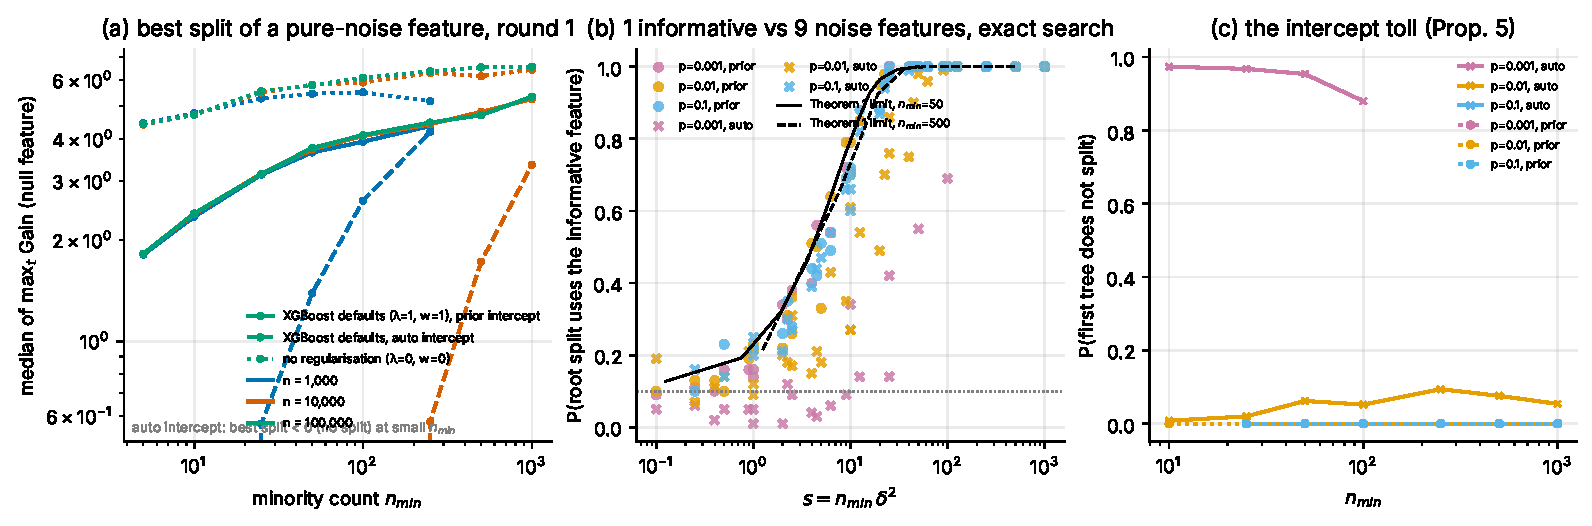
\includegraphics[width=\textwidth]{fig1_first_split}
\caption{The first split against \cref{thm:limit}. (a) Median best split of a null feature, by $n$. With XGBoost's regularisation it depends on $\nmin$ and not on $n$; without it, it grows with $n$. (b) Probability that the root uses the informative feature rather than one of nine null features (exact search, prevalence intercept), against $s = \nmin\delta^2$; error bars are two binomial standard errors. Black: the limit \eqref{eq:limit}, without fitted parameters. Dotted: chance, 1/10.}\label{fig:first}
\end{figure}

% E2, E8 and the level experiments follow once the full runs finish.
\subsection{The full ensemble}\label{sec:exp-ensemble}

\subsection{The level of the shadow rule}\label{sec:exp-level}

\section{Selection methods at both error rates}\label{sec:methods}

A method that lowers the bar loses fewer relevant features and keeps more irrelevant ones, so methods must be compared at both error rates. E4 puts 5 relevant candidates ($\delta = 0.5$, so $s = \nmin/4$) and 5 irrelevant ones in each data set; every shadow-based method builds its own $K = 10$ shadows (one permuted copy of each candidate), and all methods see the same 240 data sets ($\nmin$ from 10 to 500, $\phat\in\{0.01, 0.1\}$, 20 repeats). \Cref{tab:methods} gives both error rates, averaged over the two prevalences, and \cref{fig:methods} shows the main methods with their uncertainty. One-shot rules share the level $1/(K+1) = 0.091$ (\cref{prop:level}); their measured false positive rates, 0.08--0.09 pooled (row P9 of \cref{tab:agreement}), make their false negative rates directly comparable.

\begin{table}[t]
\centering\small
\caption{FNR / FPR by method and minority count ($\delta = 0.5$; 300-tree XGBoost unless stated; $K = 10$ shadows; 40 data sets per entry, standard errors at most 0.05 for FNR and 0.05 for FPR). The last column is the median wall time in seconds on one core at $\nmin = 100$; Boruta-style rounds cost about 20 one-shot fits.}\label{tab:methods}
\setlength{\tabcolsep}{4pt}
\begin{tabular}{@{}lcccccr@{}}
\toprule
Method & $\nmin = 10$ & 25 & 50 & 100 & 250 & s\\
\midrule
\csname @@input\endcsname generated/table_methods 
\bottomrule
\end{tabular}
\end{table}

\begin{figure}[t]
\centering
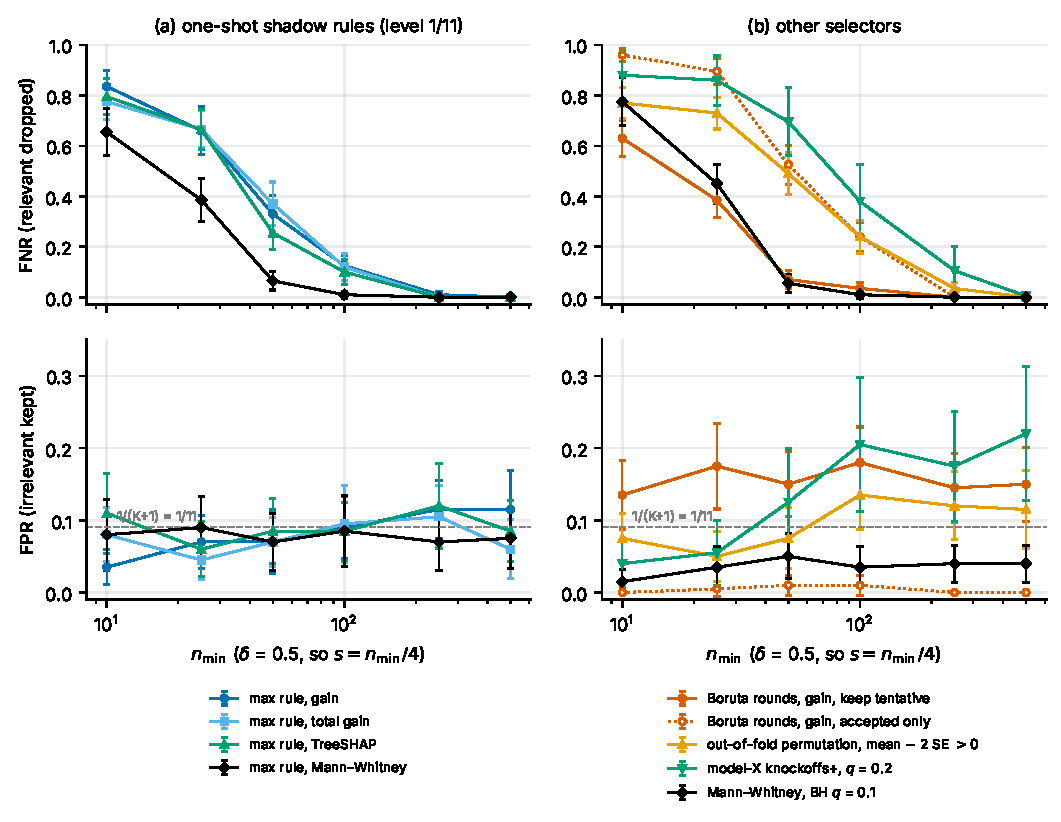
\includegraphics[width=\textwidth]{fig3_methods}
\caption{Both error rates by method ($\delta = 0.5$, the same 240 data sets for every method). Top: relevant candidates dropped; bottom: irrelevant candidates kept, with the level $1/(K+1)$ of the one-shot rules dashed. (a) One-shot max-shadow rules with three tree importances and with the Mann--Whitney statistic. (b) Other selectors. Error bars: two standard errors, clustered by data set.}\label{fig:methods}
\end{figure}

What the comparison shows:
\begin{enumerate}
  \item \emph{The importance measure matters little.} Mean gain, total gain and mean absolute TreeSHAP give the same false negative rate within two standard errors at every $\nmin$ (0.66, 0.67 and 0.67 at $\nmin = 25$). BorutaSHAP's statistic does not escape the minority-count limit.
  \item \emph{At the same level, the rank statistic loses far fewer relevant features.} With the same shadow rule, Mann--Whitney drops 0.38 of the relevant candidates at $\nmin = 25$ and 0.06 at $\nmin = 50$, against 0.66 and 0.33 for the gain. This is what \cref{cor:efficiency} and the scanning cost predict for location shifts, and the size matches \cref{prop:mw} (P13).
  \item \emph{Out-of-fold permutation importance is not more powerful.} Requiring the mean importance over five folds to exceed two standard errors keeps irrelevant candidates at the one-shot level but drops more relevant ones (0.49 at $\nmin = 50$); requiring only a positive mean keeps 0.4--0.6 of the irrelevant ones.
  \item \emph{Model-X knockoffs control false discoveries but are weak here.} With the knockoff+ threshold at $q = 0.2$ they drop 0.70 of the relevant candidates at $\nmin = 50$; the offset-free threshold has more power and an FPR near 0.3. With 10 candidates the knockoff filter has little room to work, which \cref{sec:widetables} revisits with 100 candidates.
  \item \emph{Penalised regression trades one error for the other.} Cross-validated $\ell_1$-logistic regression keeps almost every relevant candidate and 0.6--0.8 of the irrelevant ones. Stability selection with the error bound $\E V \le 1$ and threshold 0.6 selects almost nothing: with $d = 10$ candidates the bound allows only $q = \sqrt{(2\cdot 0.6-1)\,d\,\E V} \approx 1.4$ features per subsample \citep{meinshausen2010stability}, so with five relevant candidates none reaches selection probability 0.6.
  \item \emph{Boruta-style rounds help only if tentative features are kept.} Keeping tentative features drops 0.07 at $\nmin = 50$ at an FPR of about 0.15; keeping only accepted features drops 0.53 at an FPR near zero. Both match \cref{prop:rounds}: with $R = 20$ rounds, $K = 10$ and $d = 10$ the keep rate of a null candidate is about 0.10 when its hit rate does not vary, and its variation between data sets adds the rest (P12).
  \item \emph{Class weights, downsampling and early stopping do not help}, as the theory predicts: none changes $\nmin$, and downsampling the majority class to 1:1 removes information.
\end{enumerate}

% BorutaPy and the wide-table experiment (E4c, E4w) follow once the runs finish.
\subsection{Wide tables}\label{sec:widetables}

\subsection{Departures from the Gaussian model}\label{sec:robustness}

\subsection{Real data}\label{sec:realdata}

\section{Guidance}\label{sec:guidance}

The rules below follow from the results above. Each names the evidence it rests on.

\begin{enumerate}[label=\textbf{Rule \arabic*.},leftmargin=*,align=left]
  \item \emph{Count the positives in the data the selector sees.} The minority count, not the prevalence, sets what can be found (\cref{thm:limit}). With cross-validation or a held-out split, count the positives in the training part only, and run the selection inside each fold, so that the model's performance is estimated on data the selection never saw.
  \item \emph{Translate $\nmin$ into the smallest effect that can be found.} A feature's chance of beating the shadows is governed by $s = \nmin\delta^2$, or by $\sauc = 4\pi\nmin(\AUC - \frac12)^2$ for a feature of any distribution (\cref{sec:rank}). \Cref{tab:sbands} gives the false negative rate of the one-shot rule with five shadows in E2; with more shadows it is higher (\cref{cor:shadows}). A feature with single-feature ROC area 0.6 has $\sauc \approx 0.13\,\nmin$, so it is found reliably only with several hundred positives.
  \item \emph{With XGBoost before 3.0, set the intercept to the prevalence} (\code{base\_score = y.mean()}). The default of versions 1.x and 2.x adds a toll of order $\lambda/\phat$ to every split (\cref{prop:toll}) and raised the false negative rate by \numGapMeanSmall{} on average at $\phat \le 0.01$ in E2.
  \item \emph{Use a fixed, moderate number of shadows.} The level is $1/(K+1)$ whatever the imbalance (\cref{prop:level}), and more shadows cost power (\cref{cor:shadows}). Ten shadows give a level of 0.09 per one-shot comparison; one shadow per candidate, as Boruta does, makes wide tables harder than narrow ones. For discrete columns use per-feature shadows, which keep the level for any column type.
  \item \emph{Screen with a rank test.} At the same level, the Mann--Whitney test lost far fewer relevant features than any tree importance when the signal shifts the class distributions (\cref{tab:methods}), and its power is predicted by $\sauc$ (\cref{prop:mw}). It misses features that act only through their spread or through interactions (\cref{sec:robustness}), so use it to decide what is clearly in, not to drop what a model finds useful.
  \item \emph{With repeated rounds, keep the tentative features, and know the price.} Below about 100 positives, keeping only accepted features drops most moderately predictive ones (0.53 at $\nmin = 50$, $\delta = 0.5$). Keeping tentative features loses few (0.07) but keeps irrelevant candidates at a rate that depends on the number of rounds $R$, the number of shadows $K$ and the number of candidates $d$ (\cref{prop:rounds}); compute it for your $(R, K, d)$ before trusting the selection.
  \item \emph{Do not expect class weights, downsampling or early stopping to help.} None changes $\nmin$, and none helped in E4.
  \item \emph{Below about 25 positives, do not prune on importance.} At $\nmin = 10$ every method we tested either lost most relevant features or kept many irrelevant ones, and at $\nmin = 25$ the best of them, the rank test with Benjamini--Hochberg at $q = 0.2$, still lost 0.24 of the relevant features while keeping 0.15 of the irrelevant ones (\cref{tab:methods}). Keep features on domain grounds, inspect a penalised model's regularisation path, or collect more positives: doubling $\nmin$ helps as much as a feature with a $\sqrt2$ larger effect.
\end{enumerate}

\begin{table}[t]
\centering\small
\caption{False negative rate of the one-shot max-shadow rule ($K = 5$, 300-tree XGBoost, prevalence intercept) by band of $s = \nmin\delta^2$, over the E2 cells in each band.}\label{tab:sbands}
\begin{tabular}{@{}lcccl@{}}
\toprule
$s$ & range over cells & median & cells & example\\
\midrule
\csname @@input\endcsname generated/table_sbands
\bottomrule
\end{tabular}
\end{table}

\paragraph{The package.} \pkg{} implements these rules as scikit-learn compatible estimators. \code{assess\_imbalance} reports $\nmin$ and the smallest detectable effect; \code{UnivariateScreen} runs the rank-test screen with Benjamini--Hochberg control; and \code{ShadowFeatureSelector} runs Boruta-style rounds with any classifier, with ten shadows drawn afresh each round, tentative features kept, a Bonferroni or Benjamini--Hochberg correction, and the prevalence intercept set automatically for XGBoost before 3.0. It warns when the training data hold fewer than 100 positives, refuses a number of rounds too small for any feature to reach significance, and reports each feature's estimated $s$ and the expected keep rate of an irrelevant candidate for the chosen $(R, K, d)$.

\section{Limitations}\label{sec:limitations}

\paragraph{What is proved.} The limit theorems concern the first tree of a boosted ensemble with exact search; histogram search is covered under an assumption on XGBoost's quantile sketch that we have not proved. \Cref{thm:scaling} restricts thresholds to a fixed window, and the behaviour on XGBoost's full window is \cref{conj:drift}. The level results (\cref{prop:level,prop:rounds}) hold for any rank-based learner and any number of trees, but only for strong nulls: a feature that is irrelevant yet correlated with a relevant one is not covered. The power of the shadow rule on a full ensemble is \cref{conj:ensemble}, which the experiments support cell by cell but which we have not proved. \Cref{thm:limit} gives no rate of convergence.

\paragraph{What the experiments cover.} The main sweeps use Gaussian location shifts with conditionally independent features; \cref{sec:robustness} departs from this in eight ways, and \cref{sec:realdata} uses five real tables in which only the appended null columns are known to be irrelevant, so the false negative rates there rest on a pseudo-truth. We study binary targets; a rare class in a multi-class problem reduces to the same quantities one-versus-rest, but we have not tested it. The residual effect of the prevalence at fixed $\nmin$ is small but detectable at weak signal (\cref{sec:exp-ensemble}), and we have no quantitative account of it. Behaviour that depends on library defaults, such as XGBoost's intercept, is specific to the versions we name.

\section{Conclusion}\label{sec:conclusion}

The shadow rule asks whether a feature does better than the best that noise can do. With a rare positive class, how much evidence a feature can show is set by the number of positives and its effect size, through $s = \nmin\delta^2$ or its rank analogue $\sauc$, while the best that noise can do depends on $\nmin$ alone and grows only slowly. The rule's false positive level is unaffected by imbalance; its power is what imbalance removes. For the first tree this is proved, and for full ensembles the experiments find failure rates at least as high as the root-split theory predicts. Two practical consequences follow. Much of what looks like an imbalance effect in XGBoost~1.x and 2.x is the default intercept, which XGBoost~3 has removed and which one argument fixes in earlier versions. And when positives are few, a rank test on each feature uses the same information more efficiently than a tree split and does not pay for a threshold search, at the price of missing signals that only a model can see. Below about 25 positives no method we tested separates weak signal from noise reliably, and the honest answer is to keep features on domain grounds or to collect more positives.


\bibliography{references}
\bibliographystyle{tmlr}

\clearpage
\appendix
\setcounter{figure}{0}\renewcommand{\thefigure}{A\arabic{figure}}
\setcounter{table}{0}\renewcommand{\thetable}{A\arabic{table}}
\section{Proofs}\label{app:proofs}

Notation: $m = \nmin$; $\mathcal N(\mu,1)$ is the normal law; $\varphi$ and $\Phi$ are the standard normal density and distribution function; $\psi(u) = \varphi(\Phi^{-1}(u))$; $\|\cdot\|$ is the supremum norm.

\subsection{Proof of \texorpdfstring{\cref{prop:toll}}{the intercept toll}}\label{app:proof-toll}

For a child $c$ let $D_c = G_c - rH_c = -(k_c - \phat\,n_c)$. We first show the exact identity
\begin{equation}\label{eq:toll}
  \Gain = \sum_{c\in\{L,R\}} \frac{(D_c - r\lambda)^2}{H_c + \lambda} - \lambda r^2\,\frac{H + 2\lambda}{H+\lambda}.
\end{equation}
Write $G_c = rH_c + D_c = r(H_c+\lambda) + (D_c - r\lambda)$ and expand: $G_c^2/(H_c+\lambda) = r^2(H_c+\lambda) + 2r(D_c - r\lambda) + (D_c - r\lambda)^2/(H_c+\lambda)$. Summing over the two children and using $D_L + D_R = 0$ and $H_L + H_R = H$ gives $r^2H - 2\lambda r^2 + \sum_c (D_c-r\lambda)^2/(H_c+\lambda)$. The parent term is $(rH)^2/(H+\lambda) = r^2H - \lambda r^2H/(H+\lambda)$. Subtracting gives \eqref{eq:toll}.

For the approximation, $\sum_c D_c^2/H_c$ is the right-hand side of \cref{prop:chi2} at the root, $\kappa X^2$ with $\kappa = \phat(1-\phat)/(b(1-b))$. Expanding the squares in \eqref{eq:toll}, the gain minus $(\kappa X^2 - \lambda r^2)$ is the sum of four terms: $-\sum_c D_c^2\lambda/(H_c(H_c+\lambda))$, $-2r\lambda\sum_c D_c/(H_c+\lambda)$, $r^2\lambda^2\sum_c 1/(H_c+\lambda)$ and $-\lambda^2r^2/(H+\lambda)$. With $H_{\min} = \min(H_L, H_R)$, and since $D_c/H_c = (\phat - \phat_c)/(b(1-b))$ and $r = (b-\phat)/(b(1-b))$, bounding each term gives
\begin{equation}\label{eq:remainder}
  \bigl|\Gain - (\kappa X^2 - \lambda r^2)\bigr| \le \frac{\lambda}{H_{\min}}\bigl(\kappa X^2 + 2\lambda r^2\bigr) + 2\lambda r^2\sum_c \frac{|\phat_c - \phat|}{|b-\phat|},
\end{equation}
which is small when $H_c \gg \lambda$ and $|\phat_c - \phat| \ll |b - \phat|$. Solving $\kappa X^2 - \lambda r^2 > 0$ for $X^2$ gives \eqref{eq:threshold}; the asymptotic forms use $b \to \sigma(-2)$, $b/(1-b) \to e^{-2}$ (version 2.x) and $b = 1/2$ (version 1.x). \hfill$\square$

\subsection{Proof of \texorpdfstring{\cref{thm:limit}}{Theorem 1}}\label{app:proof-limit}

\emph{Coupling.} The claim is about laws, so we may build all sample sizes on one probability space. For one feature, fix the $m$ positive values $Z_1,\dots,Z_m$, i.i.d.\ with distribution $F_1$, and an infinite i.i.d.\ sequence $\xi_1, \xi_2, \dots$ with distribution $F_0$; the sample of size $n$ consists of the positives and $\xi_1, \dots, \xi_{n-m}$. Different features use independent copies, which gives independence across features at every $n$ because features are conditionally independent given $Y$. We show almost-sure convergence, which implies convergence in distribution.

\emph{Rank fractions.} Let $F^-_n$ be the empirical distribution function of $\xi_1,\dots,\xi_{n-m}$. The rank fraction of positive $i$ among all $n$ values is $\rho_i^n = n^{-1}[(n-m)F^-_n(Z_i) + \#\{l \le m : Z_l \le Z_i\}]$, so
\[
  |\rho^n_i - F_0(Z_i)| \le \|F^-_n - F_0\| + 2m/n \to 0 \quad\text{a.s.}
\]
by the Glivenko--Cantelli theorem. Let $V_i = F_0(Z_i)$. Because $V$ has no atoms, almost surely the $V_i$ are distinct, lie in $(0,1)$ and differ from $a = w/m$ and $1-a$.

\emph{The counting process.} Exact greedy search evaluates, for $j = 1,\dots,n-1$, the split that sends the $j$ smallest values left, so $u = j/n$ and $k_L(j/n) = N_n(j/n)$ with $N_n(u) = \#\{i : \rho_i^n \le u\}$. Fix $\omega$ outside a null set and $n$ large enough that the $\rho^n_i$ are in the same order as the $V_i$. Let $\ell_n$ be the increasing piecewise-linear bijection of $[0,1]$ with $\ell_n(0) = 0$, $\ell_n(1) = 1$ and $\ell_n(\rho^n_i) = V_i$. Then $N_n = N\circ\ell_n$ exactly, with $N(u) = \#\{i : V_i \le u\}$, and $\|\ell_n - \mathrm{id}\| \le \max_i|\rho^n_i - V_i| \to 0$.

\emph{The bracket.} With the prevalence intercept, $H_L = n_L\phat(1-\phat) = mu(1-\phat)$, so the admissible thresholds are $u \in [a_n, 1-a_n]$ with $a_n = w/(m(1-\phat)) \to a$, and the bracket of \eqref{eq:process} is $\beta_n(u) = [mu(1-\phat)+\lambda]^{-1} + [m(1-u)(1-\phat)+\lambda]^{-1}$. Since $w > 0$, $\beta_n \to \beta$ uniformly on $[a/2, 1-a/2]$, where $\beta$ is the bracket of \eqref{eq:limit}, and $\beta$ is uniformly continuous there (this covers $\lambda = 0$).

\emph{Process convergence.} Extend $\Gamma$ by \eqref{eq:limit} to $[a/2, 1-a/2]$. Since $N_n = N\circ\ell_n$ with $\|\ell_n - \mathrm{id}\|\to 0$, the counting processes converge in $D[0,1]$ with the $J_1$ topology \citep{billingsley1999convergence}. For the gains, on $[a_n, 1-a_n]$, $\Gain_n(u) - \Gamma(\ell_n(u)) = (N(\ell_n u) - mu)^2\beta_n(u) - (N(\ell_n u) - m\ell_n u)^2\beta(\ell_n u)$. Since $0 \le N \le m$, $|mu - m\ell_n u| \le m\|\ell_n - \mathrm{id}\|$, $\beta_n \to \beta$ uniformly and $\beta$ is uniformly continuous, $\sup_{u\in[a_n,1-a_n]}|\Gain_n(u) - \Gamma(\ell_n(u))| \to 0$.

\emph{Suprema.} The search maximises over the grid $T_n = \{j/n\}\cap[a_n, 1-a_n]$, whose image $\ell_n(T_n)$ has mesh tending to zero and end points tending to $a$ and $1-a$. $\Gamma$ is continuous except for finitely many jumps at the $V_i$, none at $a$ or $1-a$. Lower bound: the supremum of $\Gamma$ over $[a,1-a]$ is a value at a continuity point or a one-sided limit at a jump, and every open interval inside $[a,1-a]$ eventually contains points of $\ell_n(T_n)$, so $\liminf_n\max_{T_n}\Gain_n \ge \sup_{[a,1-a]}\Gamma$. Upper bound: for any $\eta > 0$, eventually $\ell_n(T_n)\subset[a-\eta, 1-a+\eta]$, so $\limsup_n\max_{T_n}\Gain_n \le \sup_{[a-\eta,1-a+\eta]}\Gamma$; let $\eta\to 0$ using the continuity of $\Gamma$ at $a$ and $1-a$. Hence $\max_{T_n}\Gain_n \to \sup_{[a,1-a]}\Gamma$ almost surely, jointly over the independently generated features, and the law of $\Gamma$ is a function of $(m, G, \lambda, w)$ only. \hfill$\square$

\begin{lemma}[shadows in the limit]\label{lem:shadow}
Let a shadow be a uniformly random row-permutation, independent of the data, of a candidate column whose negatives are i.i.d.\ from a continuous $F_0$. In the coupling above, the shadow's placements converge almost surely to i.i.d.\ uniform variables independent of the limits of all candidates and of other shadows, so its gain process converges to that of a null feature, independently of the others.
\end{lemma}

\begin{proof}
With probability at least $1 - m^2/(n-m)$ the permutation sends every positive row to a row that is negative in the source column, so the shadow's $m$ ``positive'' values are $m$ draws without replacement from the source's i.i.d.\ $F_0$ negatives, at positions chosen independently of the data; they are therefore i.i.d.\ $F_0$ and independent of the source's positives. The shadow's ``negative'' values are the source's values with $m$ of the negatives replaced by its $m$ positives, so their empirical distribution function is within $2m/(n-m)$ of the source's negative one in the supremum norm and converges uniformly to $F_0$. The argument of the proof above then gives placements $F_0(\xi)$, i.i.d.\ uniform. Distinct shadows use independent permutations, so their selected rows are disjoint with probability tending to one, and their limits are independent of each other and of the candidates' positives.
\end{proof}

\subsection{Proof of \texorpdfstring{\cref{prop:fixed}}{Proposition 3}}\label{app:proof-fixed}

$N(u)$ counts the i.i.d.\ placements with $V_i \le u$, each with probability $G(u)$, so it is binomial. $\E(N - mu)^2 = mG(1-G) + m^2(G-u)^2$; dividing by $mu(1-u)$ gives the mean. If $\sqrt m(G_m(u) - u) \to -c$ then $G_m(u)\to u \in (0,1)$, so $(N - mG_m)/\sqrt{mG_m(1-G_m)} \Rightarrow \mathcal N(0,1)$ by the de Moivre--Laplace theorem for triangular arrays, and $(mG_m - mu)/\sqrt{mu(1-u)} \to -c/\sqrt{u(1-u)}$.

For \eqref{eq:twopi}, write $x = \Phi^{-1}(u)$ and $f_\delta(x) = (\int_0^1\varphi(x-\theta\delta)\,d\theta)^2/(\Phi(x)(1-\Phi(x)))$, so that $\nu(u)/(m\delta^2) = f_\delta(x)$ by the mean value theorem. For $|\delta|\le 1$, $\varphi(x-\theta\delta) \le \varphi(x)e^{|x|}$, so $f_\delta \le g$ with $g(x) = \varphi(x)^2e^{2|x|}/(\Phi(x)(1-\Phi(x)))$, and by symmetry and the Mills-ratio bound $1-\Phi(x) \ge \varphi(x)x/(1+x^2)$, $g(x)\to 0$ as $|x|\to\infty$. On compacts $f_\delta \to f_0$ uniformly, so $\sup f_\delta \to \sup f_0$ with $f_0(x) = \varphi(x)^2/(\Phi(x)(1-\Phi(x)))$. For independent standard normals $Z_1, Z_2$ and $x\neq 0$, $(2\Phi(x)-1)^2 = \P(|Z_1|\le|x|, |Z_2|\le|x|) < \P(Z_1^2+Z_2^2 \le 2x^2) = 1 - e^{-x^2}$, because the square lies strictly inside the disc of radius $|x|\sqrt2$. Hence $\Phi(x)(1-\Phi(x)) = \frac14[1-(2\Phi(x)-1)^2] > \frac14 e^{-x^2}$ and $f_0(x) < (e^{-x^2}/2\pi)/(e^{-x^2}/4) = 2/\pi = f_0(0)$. As $f_0$ is continuous with a unique maximiser and $f_\delta\to f_0$ uniformly on compacts under the envelope $g$, every maximiser of $f_\delta$ tends to $0$, that is $u\to 1/2$. \hfill$\square$

\subsection{Proof of \texorpdfstring{\cref{thm:scaling}}{Theorem 2}}\label{app:proof-scaling}

Fix one feature with shift $\delta = \delta_m$ and $s_m = m\delta_m^2\to s$. Let $U_i = \Phi(Z_i - \delta)$, i.i.d.\ uniform. Then $\Phi(Z_i)\le u$ if and only if $U_i \le q_\delta(u) = \Phi(\Phi^{-1}(u)-\delta)$, so $N(u) = m\hat G_m(q_\delta(u))$ with $\hat G_m$ the empirical distribution function of the $U_i$. With the uniform empirical process $\alpha_m(t) = \sqrt m(\hat G_m(t) - t)$,
\[
  \frac{N(u) - mu}{\sqrt m} = \alpha_m(q_\delta(u)) + \sqrt m\,(q_\delta(u) - u).
\]
(a) \emph{Drift.} With $x = \Phi^{-1}(u)$, $u - q_\delta(u) = \delta\int_0^1\varphi(x-\theta\delta)\,d\theta$ and $|\varphi'|\le\varphi(1)$, so $|\sqrt m(u-q_\delta(u)) - \sqrt m\delta\psi(u)| \le \varphi(1)s_m/\sqrt m \to 0$ uniformly in $u$, and the drift converges uniformly to $-\sqrt s\,\psi(u)$.
(b) \emph{Noise.} $\|q_\delta - \mathrm{id}\| \le \varphi(0)\delta\to 0$. The uniform empirical process converges to a Brownian bridge $\mathbb B$ in $D[0,1]$ and is asymptotically equicontinuous \citep{shorack1986empirical,billingsley1999convergence}, so $\|\alpha_m\circ q_\delta - \alpha_m\|\to 0$ in probability and $\alpha_m\circ q_\delta\Rightarrow\mathbb B$; since the limit is continuous, the convergence holds in the supremum norm.
(c) \emph{Bracket.} On $[\varepsilon,1-\varepsilon]$, $m[(mu+\lambda)^{-1} + (m(1-u)+\lambda)^{-1}] \to 1/(u(1-u))$ uniformly. Combining (a)--(c) with the continuous mapping theorem, $\Gamma_{\delta_m}\Rightarrow\Gamma^{(s)}$ uniformly on the window; independent features give independent limits.
(d) \emph{Win probability.} $f\mapsto\sup_{[\varepsilon,1-\varepsilon]}f$ is continuous for the supremum norm, so the suprema converge jointly. For $s = 0$, $\sup\Gamma^{(0)} = (\sup_u|\mathbb B(u)|/\sqrt{u(1-u)})^2$. By Tsirelson's theorem \citep{tsirelson1975density,lifshits1995gaussian} applied to the symmetrised centred Gaussian family $\{\pm\mathbb B(u)/\sqrt{u(1-u)}\}$, the law of its supremum has no atoms except possibly at the left end of its support, which is $0$ and carries no mass. So the null suprema have continuous laws, ties have probability zero, and the win probability converges by the portmanteau theorem.
(e) \emph{Monotonicity.} For $c > 0$ let $A_c = \{f\in C[\varepsilon,1-\varepsilon] : |f(u)|\le\sqrt{c\,u(1-u)}\ \forall u\}$, a closed, convex, symmetric set, so $\P(\sup\Gamma^{(s)}\le c) = \P(\mathbb B - \sqrt s\psi\in A_c)$. The law $\gamma$ of $\mathbb B$ is a centred Gaussian Radon measure, hence log-concave \citep{borell1974convex,bogachev1998gaussian}, and $t\mapsto\gamma(A_c + t\psi)$ is log-concave and even, hence non-increasing for $t\ge 0$ (Anderson's inequality, \citealp{anderson1955integral}). So $\sup\Gamma^{(s)}$ is stochastically non-decreasing in $s$, and $\omega_\varepsilon(s,K)$ is non-decreasing in $s$.
(f) For $s = 0$ the $K+1$ suprema are i.i.d.\ with a continuous law, so each is the largest with probability $1/(K+1)$.

\emph{General local alternatives.} The argument uses the Gaussian model only in (a). If instead $\sqrt m(u - G_m(u))\to h(u)$ uniformly on the window for a continuous $h$, represent the placements as $V_i = G_m^{-1}(U_i)$ with $U_i$ i.i.d.\ uniform, so that $V_i\le u$ if and only if $U_i\le G_m(u)$ and $N(u) = m\hat G_m(G_m(u))$, with $\hat G_m$ the empirical distribution function of the $U_i$. Then $(N(u)-mu)/\sqrt m = \alpha_m(G_m(u)) + \sqrt m(G_m(u)-u)$; step (b) needs only $\|G_m - \mathrm{id}\|\to 0$, which holds on the window, and the limit is $(\mathbb B(u) - h(u))^2/(u(1-u))$. Steps (d)--(f) hold with $\sqrt s\,\psi$ replaced by $h$, and (e) gives monotonicity along $h \mapsto t h$, $t \ge 0$. \hfill$\square$

\subsection{Proof of \texorpdfstring{\cref{prop:level}}{Proposition 4}}\label{app:proof-level}

By (A0), (A3) and the strong null, the rank vector of $X_j$ is uniform over permutations and independent of $Y$ and the other candidates; by (A1) the importances depend on the columns only through such rank vectors. (A3) is needed only for $X_j$ and the shadows' source columns. A shadow's rank vector is the rank vector of its source composed with an independent uniform permutation, so it is again uniform and independent of everything else, as is the rank vector of an i.i.d.\ continuous noise column. So the rank vectors of $X_j$ and of the $K$ shadows are i.i.d.\ and independent of $Y$ and the remaining columns, and by (A2) the $K+1$ importances are exchangeable; each is the strict maximum with probability at most $1/(K+1)$. For per-feature shadows, (A0) and the strong null give $X_j = \tau x$ for its multiset of values $x$ and a uniform permutation $\tau$ independent of $(Y, X_{C\setminus j})$; the shadows are $\tau_k x$ with $\tau_k = \varrho_k\tau$ for the shadows' independent uniform permutations $\varrho_k$, and $\tau, \tau_1, \dots, \tau_K$ are i.i.d.\ uniform. The $K+1$ columns are therefore exchangeable given the rest, and (A2) gives exchangeable importances without (A1) or (A3); ties, as with discrete columns, only make the inequality strict. Shadows of other candidates do no harm, being independent of the $\varrho_k$. \hfill$\square$

\subsection{Proof of \texorpdfstring{\cref{prop:rounds}}{Proposition 5}}\label{app:proof-rounds}

Given $D$ the rounds are i.i.d., which gives the binomial law, and $\E\,\theta_j(D) = \P(\text{hit}) \le 1/(K+1)$ by \cref{prop:level} applied to each round (fresh shadows and a fresh column order make each round satisfy its conditions). The bound in \eqref{eq:rounds} is Markov's inequality for $T_j$: $\P(T_j \ge r_R+1)\le \E T_j/(r_R+1)$. As $R\to\infty$, $r_R/R\to 1/2$ and $T_j/R\to\theta_j(D)$ almost surely given $D$; for $\theta < 1/2$, $\P(\Bin(R,\theta) > r_R)\to 0$, so by dominated convergence $\limsup_R\P(\text{keep})\le\P(\theta_j(D)\ge 1/2)$. Markov's inequality for $\theta_j^2$ gives $\P(\theta_j\ge 1/2)\le 4\E\theta_j^2 = 4\operatorname{Var}\theta_j + 4(\E\theta_j)^2$, and Markov's inequality for $\theta_j$ gives $\P(\theta_j\ge 1/2)\le 2\E\theta_j\le 2/(K+1)$. \hfill$\square$

\subsection{Proof of \texorpdfstring{\cref{prop:mw}}{Proposition 6} and \texorpdfstring{\cref{cor:efficiency}}{Corollary 2}}\label{app:proof-mw}

Without ties, $U$ counts the (positive, negative) pairs with the positive larger, so $W_n = m^{-1}\sum_i F^-_n(Z_i)$ with $F^-_n$ as in \cref{app:proof-limit}. By Glivenko--Cantelli $F^-_n\to F_0$ uniformly, which gives the first form of \eqref{eq:mw}; the second follows from $\int_0^1 \mathbf 1\{V_i\le u\}\,du = 1 - V_i$.

For the normal limit, the $V_i$ form a triangular array of i.i.d.\ variables in $[0,1]$ with mean $\AUC_m$. Since the placement laws $G_m\to\mathrm{id}$ uniformly, $V_i$ converges in law to a uniform variable, and by bounded convergence $\operatorname{Var}V_i \to 1/12$. The Lindeberg--Feller theorem (the summands are bounded and their variance is bounded below) gives $\sqrt{12m}\,(W - \AUC_m)\Rightarrow \mathcal N(0,1)$. Finally $\sqrt{12m}\,(\AUC_m - \tfrac12) = \sqrt{12\,\sauc/(4\pi)}\to\sqrt{3s_*/\pi}$, and the power of the two-sided test with the null standardisation follows.

For \cref{cor:efficiency}, let $X^- \sim f$ and $X^+ = X' + \delta$ with $X'\sim f$ independent. At a fixed $u$ with $x = F^{-1}(u)$ a continuity point of $f$, $u - G_\delta(u) = F(x) - F(x-\delta) = \delta J_f(u) + o(\delta)$, so by \cref{prop:fixed} the squared mean of the standardised count is $s J_f(u)^2/(u(1-u))$ in the limit. For the rank test, $\AUC - \tfrac12 = \int [F(x+\delta) - F(x)] f(x)\,dx = \delta\int f^2 + o(\delta)$ by dominated convergence (as $f$ is bounded), so $\sauc = 4\pi s(\int f^2)^2(1+o(1))$ and its squared mean is $3\sauc/\pi = 12 s(\int f^2)^2$. Both statistics are asymptotically normal with unit variance, so the ratio of squared means is the Pitman efficiency. The numerical values in \eqref{eq:efficiency} are computed on a grid of $2\times 10^5$ points in $u$. For the normal, $J = \psi$, $\sup_u\psi^2/(u(1-u)) = 2/\pi$ and $\int\varphi^2 = 1/(2\sqrt\pi)$, so $\mathrm{ARE} = (2/\pi)/(12/(4\pi)) = 2/3$. \hfill$\square$

\section{Further theory}\label{app:theory}

\subsection{The null distribution at a fixed threshold}\label{app:nullmean}

Call a feature null if it is continuous and independent of $Y$. Given the labels, the ranks of the $\nmin$ positives among the $n$ values of a null feature are a uniformly random subset, so a split that sends a fixed number $n_L$ of samples left has $k_L\sim\mathrm{Hypergeometric}(n,\nmin,n_L)$.

\begin{proposition}[exact null mean]\label{prop:nullmean}
At the root, for a null feature, a fixed (data-independent) $n_L$, the prevalence intercept and $\lambda = 0$, $\E[\Gain] = \E[X^2] = n/(n-1)$ for every $n_L$ and every $\nmin$.
\end{proposition}

\begin{proof}
With $b = \phat$, $G = 0$, so $G_R = -G_L$ with $G_L = n_L\phat - k_L$, and $\Gain = G_L^2(1/H_L + 1/H_R) = G_L^2\,n/(\phat(1-\phat)n_Ln_R)$. Here $\E G_L = 0$ and $\operatorname{Var}k_L = n_L\phat(1-\phat)(n-n_L)/(n-1)$; substituting gives $n/(n-1)$.
\end{proof}

Imbalance therefore does not change the expected gain of a single uninformative split; it changes the \emph{shape} of its distribution. $X^2$ is approximately $\chi^2_1$ only when both children are expected to hold many positives. For a child of size $m\ll n$ holding $j$ positives, $X^2\approx(j - m\phat)^2/(m\phat)$: with $m\phat = 0.1$ and $j = 2$ it is 36, against a 99.9th percentile of 10.8 for $\chi^2_1$.

\begin{proposition}[\code{min\_child\_weight} counts expected positives]\label{prop:mcw}
In the first tree, $H_L\ge w$ means $n_L\ge w/(b(1-b))$. Under the null, a child of that size holds on average $n_L\phat\ge w\phat/(b(1-b))$ positives. With the prevalence intercept this is $w/(1-\phat)\approx w$; with the XGBoost 2.x default at $\phat = 0.001$ ($b\approx 0.12$) it is about $0.0095\,w$, a child of about 10 samples.
\end{proposition}

So XGBoost's default $w = 1$ rules out, under the prevalence intercept, the splits whose children are expected to hold fewer than about one positive, which is where the heavy tail lives; under the 2.x default it protects almost nothing. With \code{hist}, children are also unions of bins, which in practice bounds them below by roughly $n/\code{max\_bin}$ samples; this is a description of the binning, not part of the proposition.

\subsection{Signal at a fixed threshold}\label{app:fixed}

\begin{proposition}[signal at a fixed threshold]\label{prop:fixed}
In the limit of \cref{thm:limit}, $N(u) \sim \Bin(\nmin, G(u))$, and the standardised deviation $(N(u)-\nmin u)^2/(\nmin u(1-u))$, which is $\Gamma(u)$ for $\lambda = 0$, has mean $G(u)(1-G(u))/(u(1-u)) + \nu(u)$ with non-centrality $\nu(u) = \nmin (G(u)-u)^2/(u(1-u))$. If $\nmin \to \infty$ along a sequence of placement laws $G_{\nmin}$ with $\sqrt{\nmin}\,(G_{\nmin}(u) - u) \to -c$ for a fixed $u$, the standardised count $(N(u) - \nmin u)/\sqrt{\nmin u(1-u)}$ converges in law to $\mathcal N(-c/\sqrt{u(1-u)},\,1)$. In the Gaussian model,
\begin{equation}\label{eq:twopi}
  \lim_{\delta\to 0}\, \frac{\max_u \nu(u)}{\nmin\delta^2} = \frac{2}{\pi},
\end{equation}
attained at the median split $u \to 1/2$.
\end{proposition}

The proof is in \cref{app:proof-fixed}. The ratio $\varphi(x)^2/(\Phi(x)(1-\Phi(x)))$ that appears is the efficiency of dichotomising a normal sample at $x$ \citep{cox1957note}. At finite $\delta$ the best threshold moves into the positives' tail and the maximum exceeds $(2/\pi)\nmin\delta^2$, by a factor of 1.03, 1.09 and 1.47 at $\delta = 0.3$, 0.5 and 1. So $(2/\pi)s$ is the small-effect value, not an upper bound.

\subsection{Efficiency of one split relative to the rank test}\label{app:efficiency}

\begin{corollary}[efficiency of one split relative to the rank test]\label{cor:efficiency}
Let a feature follow a location family with bounded standardised density $f$, shift $\delta \to 0$ and $\nmin\delta^2 \to s$. A pre-specified threshold $u$, with $F^{-1}(u)$ uniquely defined and $f$ continuous there, has non-centrality $s\,J_f(u)^2/(u(1-u))$ (\cref{prop:fixed}), and the rank test has non-centrality $12 s\,(\int f^2)^2$ (\cref{prop:mw}, since $\AUC - \tfrac12 = \delta\int f^2 + o(\delta)$). The best fixed threshold, chosen knowing $f$, therefore has asymptotic relative efficiency
\begin{equation}\label{eq:efficiency}
  \mathrm{ARE}(f) = \frac{\sup_u J_f(u)^2/(u(1-u))}{12\,\bigl(\int f^2\bigr)^2}
\end{equation}
with respect to the rank test: $2/3$ for the normal, $3/4$ for the logistic, $0.85$ for $t_3$ and $4/3$ for the Laplace distribution (all at the median), and $4.8$ for the log-normal with $\sigma = 1$, at an interior maximiser $u \approx 0.01$ (the median split has $0.40$).
\end{corollary}

For the normal, $2/3$ is the Pitman efficiency of the median test relative to the Wilcoxon test \citep{mood1954asymptotic,hodges1956efficiency}: one fixed split needs 1.5 times as many positives as the rank test. For heavy-tailed features the gap narrows, and for strongly skewed ones a well-placed split beats the rank test; the log-normal value needs $\nmin u^* \gg 1$, so it matters only for $\nmin$ well above 100.

\subsection{Histogram search}\label{app:hist}

\begin{corollary}[histogram search]\label{cor:hist}
With \code{tree\_method="hist"} and a fixed \code{max\_bin} $= B$, suppose (H1) the cut points have empirical-CDF positions converging to $j/B$ almost surely, and (H2) no $j/B$ equals $w/\nmin$ or $1-w/\nmin$. Then the conclusion of \cref{thm:limit} holds with $u$ restricted to $\{1/B,\dots,(B-1)/B\}\cap[w/\nmin, 1-w/\nmin]$.
\end{corollary}

\begin{proof}
Under (H1) the cut $c^n_j$ has $F_n(c^n_j)\to j/B$, where $F_n$ is the empirical distribution function of all $n$ values, so $k_L$ at that cut is $N_n(F_n(c^n_j)) = N(\ell_n(F_n(c^n_j)))\to N(j/B)$, because $N$ is almost surely continuous at $j/B$. The bracket converges as before. Under (H2) each cut is eventually admissible if and only if $j/B\in(w/\nmin, 1-w/\nmin)$, so the maximum over cuts converges to the maximum of $\Gamma$ over the grid.
\end{proof}

(H1) is an assumption about XGBoost's quantile sketch. In the first tree the Hessian is constant, so the sketch is unweighted, but we have not verified (H1) analytically. Every prediction for \code{hist} in this paper is therefore conditional on it.

\subsection{The full threshold window}\label{app:conj1}

\begin{conjecture}[slow drift on the full window]\label{conj:drift}
Let $M^{(0)}_{\nmin}$ be the null supremum of \eqref{eq:limit} on the full window $[w/\nmin, 1-w/\nmin]$, with $\lambda, w > 0$ fixed, and let $\omega(s,K;\nmin)$ be the root win probability of an informative Gaussian feature with $\nmin\delta^2 = s$ against $K$ null features on that window. Then (a) $M^{(0)}_{\nmin}/(2\log\log\nmin) \to 1$ in probability as $\nmin\to\infty$; (b) at fixed $s$ and $K$, $\omega(s,K;\nmin) \to 1/(K+1)$; (c) in finite range, $\omega(12.5, 9;\nmin)$ is non-increasing in $\nmin$ and falls below 0.75 by $\nmin = 10^5$.
\end{conjecture}

The unregularised analogue: the squared supremum of the standardised uniform empirical process over $[a_m, 1-a_m]$, with $a_m \to 0$ and $m a_m \to \infty$, is $2\log\log(1/a_m)(1 + o_P(1))$ \citep{jaeschke1979asymptotic,csorgo1993weighted}. What is unproved is the regularised boundary region, where $\nmin a_{\nmin} = w$ stays bounded and the classical result does not apply. Matching the centre drift $2s/\pi$ against the null level $2\log\log\nmin$ suggests, as a heuristic, that the win probability tends to $1/(K+1)$ for $s = c\log\log\nmin$ with $c < \pi$ and to 1 with $c > \pi$, so detection at fixed power needs $s$ to grow like $\log\log\nmin$. Over the range we can compute, the median null supremum is about $1.34\times 2\log\log\nmin$, so part (a) is an asymptotic statement that the evidence does not yet reach.


Numerical evaluation of the limit \eqref{eq:limit} with $\lambda = w = 1$ and $K = 9$ null features (1{,}500 signal and 6{,}000 null draws per column; Monte Carlo standard error about 0.01):

\begin{center}\small
\begin{tabular}{lcccccc}
\toprule
$\nmin$ & 10 & 50 & 200 & 1{,}000 & 5{,}000 & 20{,}000\\
\midrule
median null supremum & 2.40 & 3.63 & 4.54 & 5.24 & 5.74 & 6.14\\
$\P$(informative wins), $s = 12.5$, full window & 0.87 & 0.85 & 0.82 & 0.79 & 0.80 & 0.76\\
\bottomrule
\end{tabular}
\end{center}

The median grows roughly like $2\log\log\nmin$ and the win probability decreases slowly; on the fixed window $[0.1, 0.9]$ the win probability is flat at $0.86\pm0.01$ for $\nmin$ from 50 to 5{,}000. The library computes these probabilities by Monte Carlo on \eqref{eq:limit} (\code{theory.detection\_probability}).

\subsection{Gain accounting for the full ensemble}\label{app:accounting}

\begin{proposition}[gain accounting]\label{prop:accounting}
Consider one tree with $\gamma = 0$ and leaves $\ell$ with gradient and Hessian sums $(G_\ell, H_\ell)$, and let $(G,H)$ be the sums over all samples. The reported gains of the tree's splits add up to
\begin{equation}\label{eq:telescope}
  \sum_{\text{splits}}\Gain = \sum_\ell\frac{G_\ell^2}{H_\ell+\lambda} - \frac{G^2}{H+\lambda}.
\end{equation}
For this tree, given its structure, with leaf values $-\eta G_\ell/(H_\ell+\lambda)$, the decrease of the second-order (Newton) approximation of the training loss is
\begin{equation}\label{eq:newton}
  \Delta\tilde L = \eta\Bigl(1-\frac\eta2\Bigr)\sum_\ell\frac{G_\ell^2}{H_\ell+\lambda} + \frac{\eta^2\lambda}{2}\sum_\ell\frac{G_\ell^2}{(H_\ell+\lambda)^2}.
\end{equation}
\end{proposition}

\begin{proof}
Each split's gain is children minus parent. Summing over internal nodes, every internal node other than the root appears once as a child and once as a parent, so the sum telescopes to \eqref{eq:telescope}. For \eqref{eq:newton}, the Newton model of the loss change is $\sum_\ell(G_\ell v_\ell + \tfrac12H_\ell v_\ell^2)$ with $v_\ell = -\eta G_\ell/(H_\ell+\lambda)$; write $H_\ell = (H_\ell+\lambda)-\lambda$ and collect terms.
\end{proof}

\emph{Heuristic consequence.} When $\lambda\ll H_\ell$ and $G\approx 0$, a tree's total gain is its Newton loss decrease divided by $\eta(1-\eta/2)$, which is 10.5 at $\eta = 0.1$ (the neglected $\lambda$ term is at most $\eta/(2-\eta)\approx 5\%$). If the Newton model approximates the true loss change, the \code{total\_gain} recorded by all features over the ensemble is about $10.5\times$ the training log-loss removed. That loss starts at $nH_2(\phat)\approx\nmin(1+\ln(1/\phat))$ nats under the prevalence intercept, where $H_2$ is the binary entropy, so more loss is available to memorise at small $\phat$. The identity concerns \code{total\_gain}; the selection statistic in most of this paper is the mean \code{gain}, and we have no argument linking the two. The measured fraction of the initial loss removed is a Newton-approximation estimate (\cref{app:agreement}, row P15).

\subsection{Keep rate of a null candidate in Boruta-style selection}\label{app:rounds-grid}

\Cref{tab:rounds-grid} evaluates $\P(\Bin(R,\pi) > r_R)$ for a constant hit rate $\pi = 1/(K+1)$, the keep rate \cref{prop:rounds} would give if the hit rate did not vary between data sets. It grows with the number of candidates $d$, because the Bonferroni threshold $r_R$ falls, and it is not monotone in $R$.

\begin{table}[h]
\centering\small
\caption{Keep rate of a null candidate under a constant hit rate $1/(K+1)$, with $K = 10$ shadows, $\alpha = 0.05$ and a Bonferroni correction over $d$ candidates, as a function of the number of rounds $R$. In parentheses: the rejection threshold $r_R$.}\label{tab:rounds-grid}
\begin{tabular}{lcccccc}
\toprule
$d$ & $R = 10$ & 18 & 20 & 40 & 60 & 100\\
\midrule
10 & 0.614 (0) & 0.074 (3) & 0.102 (3) & 0.000 (11) & 0.000 (19) & 0.000 (36)\\
50 & 0.614 (0) & 0.221 (2) & 0.272 (2) & 0.003 (9) & 0.000 (17) & 0.000 (34)\\
200 & 1.000 ($-1$) & 0.496 (1) & 0.272 (2) & 0.009 (8) & 0.000 (16) & 0.000 (32)\\
1000 & 1.000 ($-1$) & 0.820 (0) & 0.554 (1) & 0.026 (7) & 0.000 (14) & 0.000 (30)\\
\bottomrule
\end{tabular}
\end{table}

In practice the hit rate varies between data sets, and the measured keep rate at large $R$ is set by that variation (\cref{sec:methods}); the table gives the part of the keep rate that is due to the test alone.

% appendix_experiments (to be written)

% appendix_agreement (to be written)

% appendix_reproducibility (to be written)


\end{document}
